\documentclass[../../main.tex]{subfiles}
\begin{document}

\chapter{Preliminaries}\label{chap:preliminaries}

\section{Notation and Conventions}\label{sec:notation-conventions}

We work over the field $\mathbb{K}\in\{\mathbb{R},\mathbb{C}\}$. Statements that require $\mathbb{C}$ are indicated explicitly.

Vectors are column vectors unless otherwise stated. For $\mathbf{x},\mathbf{y}\in\mathbb{K}^n$ the inner product is
\[
    \langle \mathbf{x},\mathbf{y}\rangle := \mathbf{y}^H \mathbf{x},
\]
which is conjugate-linear in the first argument and linear in the second.

We define the associated Euclidean 2-norm as our standard norm $\|\cdot\| = \|\cdot\|_2$, unless otherwise specified:
\[
    \|\mathbf{x}\|_2=\sqrt{\langle\mathbf{x},\mathbf{x}\rangle}.
\]

For matrices $A\in\mathbb{K}^{m\times n}$ we use
\begin{itemize}
    \item $A^H$ for the conjugate transpose, and $A^T$ for the (real) transpose,
    \item $\overline{A}$ or $\overline{z}$ for elementwise complex conjugation,
    \item $I_n$ for the $n\times n$ identity and $0$ for a suitably sized zero matrix/vector,
    \item $A_{i,j}$ (or $[A]_{ij}$) for the $(i,j)$ entry and $A_{p:q,r:s}$ for the submatrix with row indices $p,\dots,q$ and column indices $r,\dots,s$,
    \item $\operatorname{diag}(d_1,\dots,d_n)$ for a diagonal matrix with the given diagonal entries.
\end{itemize}

Matrix norms and spectral quantities:
\[
    \|A\|_2 := \max_{\|\mathbf{x}\|_2=1}\|A\mathbf{x}\|_2 \qquad\text{(spectral/operator 2-norm)},
\]
\[
    \|A\|_F := \sqrt{\sum_{i,j}|a_{ij}|^2}\qquad\text{(Frobenius norm)},
\]
\[
    \rho(A) := \max_i |\lambda_i(A)|\qquad\text{(spectral radius)}.
\]

Other common notation:
\begin{itemize}
    \item $e_i$ denotes the $i$th standard basis vector in $\mathbb{K}^n$ and $\mathbf{e}=(1,\dots,1)^\top$,
    \item $\operatorname{tr}(A)$ denotes the trace, $\det(A)$ the determinant, and $\operatorname{rank}(A)$ the rank,
    \item $\Re(z)$ and $\Im(z)$ denote the real and imaginary parts of a complex number $z$,
    \item for sequences/functions we use standard asymptotic notation ($O(\cdot), o(\cdot)$) when needed.
\end{itemize}

These conventions are used throughout the text; any deviation will be stated where it occurs.

\section{Matrices}\label{sec:matrices}

\subsection{Eigenvalues and Eigenvectors}\label{subsec:eigs}
Let $A\in\mathbb{C}^{n\times n}$. A scalar $\lambda\in\mathbb{C}$ and nonzero vector $\mathbf{v}\in\mathbb{C}^n$ satisfy
\[
    A\mathbf{v}=\lambda\mathbf{v}\qquad\text{(right eigenpair)}.
\]
Left eigenvectors $\mathbf{w}$ satisfy $\mathbf{w}^H A = \lambda \, \mathbf{w}^H$, equivalently $A^H\mathbf{w}=\overline{\lambda}\,\mathbf{w}$. If $A$ is Hermitian ($A^H=A$), all eigenvalues are real; if $A$ is singular, $0$ is an eigenvalue.

\subsection{Image (Range) and Kernel (Nullspace)}
\label{subsec:image-kernel}

\begin{definition}{Image / Range}{image}
    The \emph{image} (or \emph{range}) of $A\in\mathbb{R}^{m\times n}$ is
    \[
        \operatorname{Im}(A)=\{A\mathbf{x}:\mathbf{x}\in\mathbb{R}^n\} =\operatorname{span}\{\mathbf{a}_1,\dots,\mathbf{a}_n\},
    \]
    where $\mathbf{a}_j$ are the columns of $A$. The \emph{rank} of $A$ is
    \[
        \operatorname{rank}(A)=\dim(\operatorname{Im}(A)).
    \]
\end{definition}

\begin{definition}{Kernel / Null space}{nullspace}
    The \emph{kernel} (or \emph{null space}) of $A\in\mathbb{R}^{m\times n}$ is
    \[
        \ker(A)=\{\mathbf{x}\in\mathbb{R}^n: A\mathbf{x}=\mathbf{0}\}.
    \]
    Its dimension is the \emph{nullity} of $A$:
    \[
        \operatorname{nullity}(A)=\dim(\ker(A)).
    \]
\end{definition}

\begin{theorem}{Rank-Nullity Theorem}{rank-nullity-theorem}
    For any matrix $A\in\mathbb{R}^{m\times n}$,
    \[
        \operatorname{rank}(A)+\operatorname{nullity}(A)=n.
    \]
\end{theorem}

\begin{proof}[Proof sketch]
    Consider the linear map $x\mapsto Ax$. Choose a basis of $\ker(A)$ and extend it to a basis of $\mathbb{R}^n$. The remaining basis vectors map to a basis of $\operatorname{Im}(A)$, giving the stated equality.
\end{proof}

Immediate consequences of the rank-nullity theorem are:
\begin{itemize}
    \item $A$ has full column rank iff $\ker(A)=\{0\}$.
    \item If $m<n$ then $\ker(A)\neq\{0\}$ for rank-deficient $A$ (pigeonhole).
    \item Solutions of $A\mathbf{x}=\mathbf{b}$ exist iff $\mathbf{b}\in\operatorname{Im}(A)$; when solutions exist they form an affine space $\mathbf{x}_0+\ker(A)$.
\end{itemize}

\subsection{Normal Matrices}
\label{subsec:normal-matrices}

A matrix $A \in \mathbb{C}^{n \times n}$ is \emph{normal} if
\[
    AA^H = A^H A,
\]
For real matrices, this becomes $AA^T = A^TA$.

Normal matrices are special because they \emph{commute} with their conjugate transpose; meaning $A A^H = A^H A$. This property guarantees that the matrix has a complete set of orthogonal eigenvectors.

\begin{remark}{Intuition for Normal Matrices}{intuition-normal-matrices}
    Think of Normal Matrices like this: most matrices will stretch, rotate, AND skew vectors in complicated ways. But normal matrices are \emph{well-behaved}, they only stretch or shrink along specific perpendicular directions, without mixing them up. This makes them much easier to understand and work with.
\end{remark}

\begin{theorem}{Spectral Theorem for Normal Matrices}{spectral-normal}
    A matrix $A \in \mathbb{C}^{n \times n}$ is normal if and only if it admits a unitary diagonalization:
    \[
        A = U D U^H,
    \]
    where $U \in \mathbb{C}^{n \times n}$ is unitary ($U^H U = I$) and $D = \text{diag}(\lambda_1, \ldots, \lambda_n)$ contains the eigenvalues.
\end{theorem}

This characterization shows that normal matrices are precisely those with a complete orthonormal basis of eigenvectors. The geometric intuition is that normal matrices preserve orthogonality when acting on their eigenspaces.

\paragraph{Important subclasses of normal matrices:}
\begin{description}
    \item[Hermitian matrices:] $A = A^H$, which implies all eigenvalues are real: $\lambda_i \in \mathbb{R}$.
    \item[Skew-Hermitian matrices:] $A = -A^H$, which implies all eigenvalues are purely imaginary: $\lambda_i \in i\mathbb{R}$.
    \item[Unitary matrices:] $A^H A = I$, which implies all eigenvalues have unit modulus: $|\lambda_i| = 1$.
\end{description}

\subsection{Hermitian Matrices}

\begin{definition}{Hermitian (Self-adjoint)}{hermitian}
    A matrix $A \in \mathbb{C}^{n \times n}$ is \emph{Hermitian}(or \emph{self-adjoint}) if
    \[
        A = A^H,
    \]
    that is, $A$ equals its conjugate transpose. Over the reals, this condition reduces to symmetry: $A = A^\top$.
\end{definition}

\begin{remark}{Intuition}{intuition-hermitian}
    Hermitian matrices are the complex analogue of real symmetric matrices.
    They have a built-in geometric symmetry: being equal to their own conjugate transpose makes them “balanced” across the main diagonal.
    This structure guarantees real eigenvalues and an orthonormal eigenbasis, which makes Hermitian matrices highly predictable and stable compared to general matrices.
\end{remark}

\begin{theorem}{Spectral Theorem for Hermitian Matrices}{spectral-hermitian}
    If $A \in \mathbb{C}^{n \times n}$ is Hermitian, then:
    \begin{enumerate}
        \item All eigenvalues are real: $\lambda_i \in \mathbb{R}$.
        \item There exists an orthonormal basis of eigenvectors.
        \item $A$ admits a unitary diagonalization:
              \[
                  A = U D U^H,
              \]
              where $U$ is unitary and $D$ is a real diagonal matrix of eigenvalues.
    \end{enumerate}
\end{theorem}

\begin{proof}[Proof sketch: eigenvalues are real]
    Let $\lambda$ be an eigenvalue of $A$ with eigenvector $\mathbf{v} \neq 0$. Then
    \[
        \lambda \|\mathbf{v}\|^2
        = \lambda \mathbf{v}^H \mathbf{v}
        = \mathbf{v}^H A \mathbf{v}
        = \mathbf{v}^H A^H \mathbf{v}
        = (A\mathbf{v})^H \mathbf{v}
        = (\lambda \mathbf{v})^H \mathbf{v}
        = \overline{\lambda}\, \|\mathbf{v}\|^2.
    \]
    Since $\|\mathbf{v}\|^2 > 0$, we conclude $\lambda = \overline{\lambda}$, hence $\lambda \in \mathbb{R}$.
\end{proof}

\paragraph{Variational characterization.}
For Hermitian $A$, the eigenvalues sorted nonincreasingly satisfy the \emph{min-max principle}:
\[
    \lambda_k(A)=\min_{\dim S=k}\ \max_{\substack{\mathbf{x}\in S\\ \|\mathbf{x}\|=1}} \mathbf{x}^H A \mathbf{x}.
\]
The Rayleigh quotient $R_A(\mathbf{x})=\dfrac{\mathbf{x}^H A \mathbf{x}}{\mathbf{x}^H \mathbf{x}}$ obeys $\min R_A=\lambda_n$, $\max R_A=\lambda_1$.

\paragraph{Computational advantages.}
Hermitian structure halves storage, enables real arithmetic when $A\in\mathbb{R}^{n\times n}$, and admits stable, cost-effective eigenvalue algorithms (e.g., tridiagonal reduction + QR). Perturbation theory is particularly benign: eigenvalues satisfy Weyl's theorem; eigenvectors obey Davis-Kahan bounds when eigenvalue gaps are present.

\begin{example}{Quadratic Forms}{quadratic-forms}
    For Hermitian $A$ and vector $\mathbf{x}$, the quadratic form $\mathbf{x}^H A \mathbf{x}$ is always real. Using the spectral decomposition:
    \[
        \mathbf{x}^H A \mathbf{x} = \mathbf{x}^H U D U^H \mathbf{x} = \sum_{i=1}^n \lambda_i |u_i^H \mathbf{x}|^2
    \]
    This shows how the eigenvalues directly control the behavior of the quadratic form.
\end{example}

The special structure of normal and Hermitian matrices makes them the foundation for many numerical algorithms, from eigenvalue computation to optimization methods that rely on their predictable spectral behavior.

\subsection{Nonnegative Matrices}
Nonnegative matrices are widely used in applications involving positive quantities, such as probability distributions, population dynamics, economic models, and network analysis. Their spectral properties are described by the Perron-Frobenius theory, which governs their eigenvalue structure.

\begin{definition}{Nonnegative Matrix}{nonnegative-matrix}
    A matrix $A \in \mathbb{R}^{n \times n}$ is \emph{nonnegative} if $a_{ij} \geq 0$ for all $i, j$. We write $A \geq 0$.

    A matrix is \emph{positive} if $a_{ij} > 0$ for all $i, j$, denoted $A > 0$.
\end{definition}

\begin{theorem}{Perron-Frobenius Theorem}{perron-frobenius}
    Let $A \geq 0$ be a nonnegative matrix. Then:
    \begin{enumerate}
        \item The spectral radius $\rho(A) = \max_i |\lambda_i|$ is an eigenvalue of $A$.
        \item There exists a nonnegative eigenvector $\mathbf{x} \geq 0$ such that $A\mathbf{x} = \rho(A)\mathbf{x}$.
        \item If $A$ is irreducible, then $\rho(A)$ is a simple eigenvalue, and there exists a positive eigenvector $\mathbf{x} > 0$ such that $A\mathbf{x} = \rho(A)\mathbf{x}$.
        \item If $A$ is irreducible and aperiodic, then $\rho(A)$ is the unique eigenvalue of maximum modulus, i.e., $|\lambda| < \rho(A)$ for all other eigenvalues $\lambda$.
    \end{enumerate}
\end{theorem}

The Perron-Frobenius theorem guarantees that nonnegative matrices have a dominant eigenvalue $\rho(A)$, which is real and positive.
This eigenvalue corresponds to a nonnegative eigenvector, and in the case of irreducibility, a strictly positive eigenvector.

The dominant eigenvalue $\rho(A)$ often represents the long-term growth rate or stability of the system described by $A$.

\subsection{Kantorovich Inequality}\label{subsec:kantorovich-inequality}

Kantorovich inequality provides bounds on the relationship between different norms induced by a symmetric positive definite matrix.
\begin{theorem}{Kantorovich Inequality}{kantorovich}
    Let $B \in \mathbb{R}^{n \times n}$ be SPD with eigenvalues $0 < \lambda_1 \leq \cdots \leq \lambda_n.$
    Then for all $\mathbf{x} \in \mathbb{R}^n$,
    \[
        \frac{\|\mathbf{x}\|_B^2 \,\|\mathbf{x}\|_{B^{-1}}^2}{\|\mathbf{x}\|_2^4}
        \leq \frac{1}{4}\cdot\frac{(\lambda_1 + \lambda_n)^2}{\lambda_1 \lambda_n}.
    \]
\end{theorem}
\begin{proof}
    Since $B$ is SPD, diagonalize $B = Q^{\top}\Lambda Q$ with $\Lambda = \operatorname{diag}(\lambda_1, \ldots, \lambda_n)$ and $Q$ orthogonal.
    For $y = Q\mathbf{x}$ with $\|\mathbf{x}\|_2 = \|y\|_2 = 1$:
    \begin{align*}
        B^{-1}                    & = Q^{\top} \Lambda^{-1} Q,                                                 \\
        \|\mathbf{x}\|_B^2        & = \mathbf{x}^{\top} B \mathbf{x} = \sum_{i=1}^n \lambda_i y_i^2,           \\
        \|\mathbf{x}\|_{B^{-1}}^2 & = \mathbf{x}^{\top} B^{-1} \mathbf{x} = \sum_{i=1}^n \lambda_i^{-1} y_i^2.
    \end{align*}

    Thus $\big(\bar\lambda, \bar\lambda^{-1}\big)$ with
    \[
        \bar\lambda = \sum_{i=1}^n \lambda_i y_i^2,
        \qquad
        \bar\lambda^{-1} = \sum_{i=1}^n \lambda_i^{-1} y_i^2,
    \]
    is a convex combination of points $(\lambda_i, 1/\lambda_i)$.

    The curve $1/\lambda$ is convex on $(0,\infty)$, hence
    \[
        \big(\bar\lambda, \bar\lambda^{-1}\big)
    \]
    lies below the chord
    \[
        \ell(\lambda) = \frac{1}{\lambda_1} + \frac{1}{\lambda_n} - \frac{\lambda}{\lambda_1 \lambda_n},
        \qquad \ell(\lambda_1) = \tfrac{1}{\lambda_1}, \;\; \ell(\lambda_n) = \tfrac{1}{\lambda_n}.
    \]
    Therefore
    \[
        \bar\lambda^{-1} \leq \ell(\bar\lambda).
    \]
    The maximum of $q(\bar\lambda) = \bar\lambda\,\ell(\bar\lambda)$ occurs at $\bar\lambda = \tfrac{1}{2}(\lambda_1 + \lambda_n)$, yielding
    \[
        \bar\lambda \,\bar\lambda^{-1} \leq \max_{\bar\lambda \in [\lambda_1, \lambda_n]} q(\bar\lambda) = \frac{(\lambda_1 + \lambda_n)^2}{4 \lambda_1 \lambda_n}
    \]\qed
\end{proof}

\begin{figure}[ht]
    \centering
    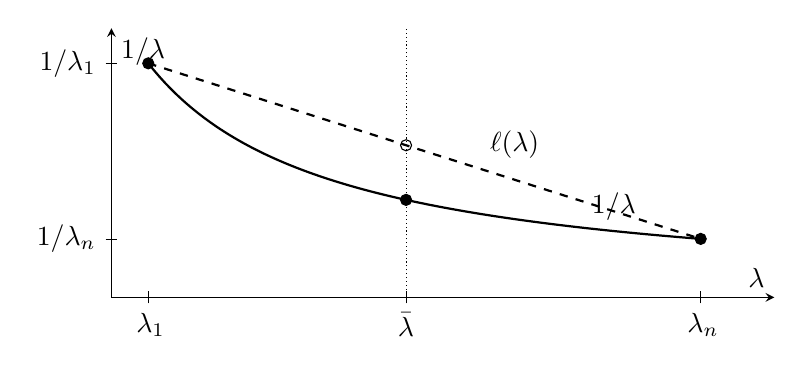
\begin{tikzpicture}
    \begin{axis}[
            width=10cm, height=6.2cm,
            axis lines=middle,
            xmin=0.8, xmax=4.4,
            ymin=0,   ymax=1.15,
            xlabel={$\lambda$}, ylabel={$1/\lambda$},
            xtick={1,2.4,4},
            xticklabels={$\,\lambda_1$, $\bar\lambda$, $\,\lambda_n$},
            ytick={1,0.25},
            yticklabels={$1/\lambda_1$, $1/\lambda_n$},
            tick style={black},
            width=10cm, height=5cm
        ]
        % curve y = 1/x
        \addplot[thick, samples=100, domain=1:4] {1/x} node[pos=0.85, above] {$1/\lambda$};

        % chord between (\lambda_1,1/\lambda_1) and (\lambda_n,1/\lambda_n)
        \addplot[thick, dashed, domain=1:4, samples=2]
        {(1/1) + ((1/4)-(1/1))*((x-1)/(4-1))}
        node[pos=0.6, above right] {$\ell(\lambda)$};

        % endpoints
        \addplot[only marks, mark=*] coordinates {(1,1) (4,0.25)};

        % bar-lambda marks
        \addplot[densely dotted] coordinates {(2.4,0) (2.4,1.2)};
        \addplot[only marks, mark=*] coordinates {(2.4,{1/2.4})}; % point on curve
        \addplot[only marks, mark=o] coordinates {(2.4,{ (1/1) + ((1/4)-(1/1))*((2.4-1)/(4-1)) })}; % point on chord

        % label
        \node[below] at (axis cs:2.4,0) {$\bar\lambda$};
    \end{axis}
\end{tikzpicture}
    \caption{Kantorovich inequality visualized via the convexity of $1/\lambda$ and its chord between $\lambda_1$ and $\lambda_n$.}
\end{figure}

\subsection{M-matrices}
M-matrices are matrices with nonpositive off-diagonal entries and a nonnegative inverse.
They ensure stability and monotonicity, making them useful in numerical analysis, optimization, and modeling problems with positivity constraints.

\begin{definition}{M-matrix}{m-matrix}
    A matrix $A \in \mathbb{R}^{n \times n}$ is an \emph{M-matrix} if:
    \begin{enumerate}
        \item $a_{ij} \leq 0$ for all $i \neq j$ (nonpositive off-diagonal entries)
        \item $A$ is nonsingular
        \item $A^{-1} \geq 0$ (nonnegative inverse)
    \end{enumerate}
\end{definition}

\begin{corollary}{M-matrix characterization}{m-matrix-characterization}
    An M-matrix can be written as $A = sI - B$ where $s > \rho(B)$ and $B \geq 0$.
\end{corollary}

\subsubsection{Properties of M-matrices}
Let $A$ be an M-matrix. Then:
\begin{enumerate}
    \item All eigenvalues have positive real parts: $\operatorname{Re}(\lambda_i) > 0$ for all $i$.
    \item All principal minors are positive: $\det(A_{ij}) > 0$ for all principal submatrices $A_{ij}$.
    \item $A$ is positive stable: solutions to $\mathbf{x}' = -A\mathbf{x}$ decay exponentially.
    \item The linear system $A\mathbf{x} = \mathbf{b}$ with $\mathbf{b} \geq 0$ has solution $\mathbf{x} \geq 0$.
\end{enumerate}

Their positive inverse property makes them particularly well-suited for iterative solution methods, as they preserve nonnegativity and ensure convergence.

\begin{example}{Discrete Laplacian as M-matrix}{discrete-laplacian}
    Consider the discrete 1D Laplacian on $n$ interior points with Dirichlet boundary conditions:
    \[
        A = \frac{1}{h^2} \begin{bmatrix}
            2  & -1 &        &        &        \\
            -1 & 2  & -1     &        &        \\
               & -1 & 2      & -1     &        \\
               &    & \ddots & \ddots & \ddots \\
               &    &        & -1     & 2
        \end{bmatrix}
    \]

    This matrix satisfies the M-matrix conditions: the diagonal entries are positive, off-diagonal entries are nonpositive, and the matrix is positive definite (hence $A^{-1} > 0$). This structure ensures that the discrete maximum principle holds for the corresponding difference equations.
\end{example}

\subsection{Unitary Matrices}

A matrix $Q \in \mathbb{C}^{n \times n}$ is \emph{unitary} if $Q^H Q = I_n$, where $I_n$ is the $n \times n$ identity matrix. The columns of $Q$ form an orthonormal set, meaning they are mutually orthogonal and each has unit norm.

Let $Q = [q_1, q_2, \ldots, q_n]$. Then the orthonormality condition is:
\begin{equation}
    (q_i, q_j) = \delta_{ij} = \begin{cases}
        1 & \text{if } i = j    \\
        0 & \text{if } i \neq j
    \end{cases}
\end{equation}

\begin{example}{Examples of Unitary Matrices}{unitary-examples}

    \begin{enumerate}
        \item \textbf{Identity matrix}: $I_n$ is trivially unitary.

        \item \textbf{2D rotation matrices} (real orthogonal):
              \begin{equation}
                  R(\theta) = \begin{bmatrix}
                      \cos(\theta) & -\sin(\theta) \\
                      \sin(\theta) & \cos(\theta)
                  \end{bmatrix}
              \end{equation}
              Verification: $R(\theta)^T R(\theta) = I_2$ since $\cos^2(\theta) + \sin^2(\theta) = 1$.

        \item \textbf{Givens rotation}: $G(i,j,\theta)$ rotates components $i$ and $j$ by angle $\theta$:
              \begin{equation}
                  G(i,j,\theta) = \begin{bmatrix}
                      I_{i-1} &   &    &         \\
                              & c & -s &         \\
                              & s & c  &         \\
                              &   &    & I_{n-j}
                  \end{bmatrix}
              \end{equation}
              where $c = \cos(\theta)$, $s = \sin(\theta)$, and the $2 \times 2$ rotation block appears at positions $(i,i)$ through $(j,j)$.

        \item \textbf{Householder reflector}: Given a unit vector $v \in \mathbb{C}^n$ with $\|v\|_2 = 1$:
              \begin{equation}
                  P = I_n - 2 v v^H
              \end{equation}
              This matrix satisfies $P = P^H = P^{-1}$ (it is Hermitian and unitary).

              \textbf{Verification of unitarity:}
              \begin{align}
                  P^H P & = (I_n - 2 v v^H)^2               \\
                        & = I_n - 4 v v^H + 4 v (v^H v) v^H \\
                        & = I_n - 4 v v^H + 4 v v^H = I_n
              \end{align}

              \textbf{Geometric interpretation:} For any vector $\mathbf{x}$:
              \begin{equation}
                  P \mathbf{x} = \mathbf{x} - 2 (v^H \mathbf{x}) v = \mathbf{x} - 2 (\mathbf{x}, v) v
              \end{equation}
              This reflects $\mathbf{x}$ across the hyperplane orthogonal to $v$.
    \end{enumerate}
\end{example}

\subsubsection{Properties of Unitary Matrices}

\begin{itemize}
    \item \textbf{Inner product preservation}: $(Q\mathbf{x}, Q\mathbf{y}) = (\mathbf{x}, \mathbf{y})$
    \item \textbf{Norm preservation}: $\|Q\mathbf{x}\| = \|\mathbf{x}\|$
    \item \textbf{Unit determinant}: $|\det(Q)| = 1$
    \item \textbf{Eigenvalues on unit circle}: All eigenvalues of $Q$ satisfy $|\lambda| = 1$
\end{itemize}

\subsubsection{Applications}
\begin{itemize}
    \item \textbf{Spectral decomposition}: If $A = A^H$, then $A = V\Lambda V^H$ where $V$ is unitary and $\Lambda$ is real diagonal.
    \item \textbf{QR decomposition}: Any matrix $A$ can be factored as $A = QR$ where $Q$ is unitary and $R$ is upper triangular.
\end{itemize}

\section{Canonical Forms and Matrix Structure}\label{sec:canonical-forms}
Canonical forms provide standardized representations that reveal the essential structure of mathematical objects. In numerical linear algebra, they serve both theoretical and computational purposes, offering insight into matrix properties and serving as targets for numerical algorithms.

\begin{definition}{Canonical Form}{canonical-form}
    A canonical form is a unique representative chosen from each equivalence class of objects under a given equivalence relation, selected according to a fixed rule or procedure.
\end{definition}

Understanding canonical forms helps us recognize when two apparently different matrices share the same fundamental properties and provides roadmaps for developing efficient algorithms.

\subsection{Similarity of Matrices}\label{subsec:similarity-of-matrices}

Two matrices $A, B \in \mathbb{C}^{n \times n}$ are \emph{similar} if there exists an invertible matrix $X$ such that
\[
    B = X^{-1} A X.
\]
Similarity defines an equivalence relation on the set of square matrices, partitioning them into equivalence classes where matrices within the same class share the same eigenvalues (counting multiplicities) and many other spectral properties.

\begin{remark}{Intuition for Similarity}{similarity-intuition}
    Similarity transformations correspond to changing the basis of the vector space. If we think of a matrix as representing a linear transformation with respect to a particular basis, then similar matrices represent the same transformation but expressed in different bases. This explains why similar matrices have the same eigenvalues: eigenvalues are invariant under basis changes.
\end{remark}

\begin{theorem}{Properties Preserved by Similarity}{similarity-properties}
    If $A$ and $B$ are similar matrices, then they share the following properties:
    \begin{enumerate}
        \item eigenvalues (including algebraic multiplicities).
        \item characteristic polynomial: $\det(\lambda I - A) = \det(\lambda I - B)$
        \item trace: $\operatorname{tr}(A) = \operatorname{tr}(B)$
        \item determinant: $\det(A) = \det(B)$
        \item rank: $\operatorname{rank}(A) = \operatorname{rank}(B)$
        \item minimal polynomial: $\mu_A(\lambda) = \mu_B(\lambda)$
    \end{enumerate}
\end{theorem}

\begin{proof}[Proof sketch]
    Most properties follow directly from the similarity transformation.

    For eigenvalues: if $A\mathbf{v} = \lambda \mathbf{v}$, then
    \begin{align*}
        B(X^{-1}\mathbf{v}) & = X^{-1} A X(X^{-1}\mathbf{v}) \\
                            & = X^{-1} A \mathbf{v}          \\
                            & = X^{-1} (\lambda \mathbf{v})  \\
                            & = \lambda X^{-1} \mathbf{v}
    \end{align*}
    The characteristic polynomial follows from the eigenvalues, and trace/determinant are polynomial functions of the eigenvalues.
\end{proof}

Canonical forms are essentially unique representatives of similarity equivalence classes, chosen according to specific rules (e.g., diagonal form for diagonalizable matrices, Jordan form for general matrices).

\subsection{Affine Spaces and Affine Maps}\label{sec:affine-spaces}

\begin{definition}{Affine subspace}{affine-subspace}
    Let $\mathbb{K}\in\{\mathbb{R},\mathbb{C}\}$. An \emph{affine subspace} of $\mathbb{K}^n$ is a translate of a linear subspace.
    For a point $\mathbf{p}\in\mathbb{K}^n$ and a linear subspace $V\subseteq\mathbb{K}^n$ the set
    \[
        \mathcal{A}=\mathbf{p}+V=\{\mathbf{p}+\mathbf{v}:\mathbf{v}\in V\}
    \]
    is an affine subspace. The subspace $V$ is called the \emph{direction} of $\mathcal{A}$.
\end{definition}

A finite set of points $\{\mathbf{x}_1,\dots,\mathbf{x}_k\}\subset\mathbb{K}^n$ is \emph{affinely independent} if the vectors
\[
    \mathbf{x}_2-\mathbf{x}_1,\ \dots,\ \mathbf{x}_k-\mathbf{x}_1
\]
are linearly independent. The \emph{affine hull} of a set $S\subset\mathbb{K}^n$, denoted $\operatorname{aff}(S)$, is the smallest affine subspace containing $S$. Equivalently,
\[
    \operatorname{aff}(S)=\Big\{\sum_{i}\alpha_i\mathbf{x}_i : \mathbf{x}_i\in S,\ \sum_i\alpha_i=1\Big\},
\]
the set of all affine combinations of points in $S$.

\begin{definition}{Affine map}{affine-map}
    An \emph{affine map} is a function $f:\mathbb{K}^n\to\mathbb{K}^m$ of the form
    \[
        f(\mathbf{x}) = A\mathbf{x} + \mathbf{b},
    \]
    where $A\in\mathbb{K}^{m\times n}$ is the linear part and $\mathbf{b}\in\mathbb{K}^m$ is a translation.
\end{definition}

Let $f(\mathbf{x})=A\mathbf{x}+\mathbf{b}$ be an affine map. Then
\begin{enumerate}
    \item $f$ preserves affine combinations; in particular, $f$ maps affine subspaces to affine subspaces.
    \item $f$ is linear if and only if $\mathbf{b}=\mathbf{0}$.
    \item The composition of two affine maps is affine.
\end{enumerate}

\subsection{Matrix Polynomials}\label{sec:polynomials}

A polynomial $p(t)=\sum_{k=0}^d c_k t^k\in\mathbb{K}[t]$ acts on a matrix $A\in\mathbb{K}^{n\times n}$ by
\[
    p(A)=\sum_{k=0}^d c_k A^k.
\]
The set $\{p(A):p\in\mathbb{K}[t]\}$ is a \emph{commutative subalgebra} of $\mathbb{K}^{n\times n}$.

\begin{remark}{commutative subalgebra}{commutative-subalgebra}
    The set
    \[
        \{p(A) : p \in \mathbb{K}[t]\} \subseteq \mathbb{K}^{n \times n}
    \]
    is a subalgebra: it contains $0$ and $I$, is closed under addition and scalar multiplication, and satisfies $(pq)(A) = p(A)q(A)$,
    so it is closed under multiplication.
    Since all elements are polynomials in the same matrix $A$, they commute, and the subalgebra is commutative.
\end{remark}



\begin{example}{Commutative subalgebra}{commutative-subalgebra}
    If $A=\begin{bmatrix}0&1\\0&0\end{bmatrix}$, then
    \[
        \{p(A):p\in\mathbb{R}[t]\}=\left\{\begin{bmatrix}c_0&c_1\\0&c_0\end{bmatrix}:c_0,c_1\in\mathbb{R}\right\}.
    \]
    This is a $2$-dimensional subalgebra of $\mathbb{R}^{2\times 2}$.
\end{example}

\paragraph{Minimal Polynomial}
The \emph{minimal polynomial} $\mu_A(t)$ of $A\in\mathbb{K}^{n\times n}$ is the unique monic polynomial of smallest degree satisfying
\[
    \mu_A(A)=0.
\]

For $A\in\mathbb{K}^{n\times n}$ the minimal polynomial $\mu_A(t)$ satisfies:
\begin{enumerate}
    \item $\mu_A$ divides every polynomial $p$ with $p(A)=0$.
    \item The distinct roots of $\mu_A$ are precisely the eigenvalues of $A$.
    \item For each eigenvalue $\lambda$, the multiplicity of $(t-\lambda)$ in $\mu_A$ equals the size of the largest Jordan block of $A$ associated with $\lambda$.
    \item $\deg(\mu_A)\le n$ and $\mu_A$ divides the characteristic polynomial $\chi_A(t)=\det(tI-A)$.
\end{enumerate}
Knowledge of $\mu_A$ determines the smallest polynomial algebra containing $A$.

\begin{example}
    If $A$ is diagonalizable with distinct eigenvalues $\{\lambda_1,\dots,\lambda_r\}$, then
    \[
        \mu_A(t)=\prod_{i=1}^r (t-\lambda_i).
    \]
\end{example}

\subsection{Jordan Canonical Form}\label{subsec:jordan-canonical-form}
Jordan form reveals the fine structure of linear transformations, particularly the behavior of eigenspaces and generalized eigenspaces.

A Jordan block of size $k$ with eigenvalue $\lambda$ is the $k \times k$ matrix
\[
    J_k(\lambda) = \begin{bmatrix}
        \lambda & 1       &        &         &         \\
                & \lambda & 1      &         &         \\
                &         & \ddots & \ddots  &         \\
                &         &        & \lambda & 1       \\
                &         &        &         & \lambda
    \end{bmatrix}.
\]
The superdiagonal of 1's captures the action on generalized eigenvectors.

Jordan blocks represent the building blocks of linear transformations that are "as close to diagonal as possible" when diagonalization is not achievable.

\begin{definition}{Jordan Canonical Form}{jordan-canonical}
    Every square matrix $A \in \mathbb{C}^{n \times n}$ is similar to a block diagonal matrix
    \[
        J = \begin{bmatrix}
            J_{k_1}(\lambda_1) &                    &        &                    \\
                               & J_{k_2}(\lambda_2) &        &                    \\
                               &                    & \ddots &                    \\
                               &                    &        & J_{k_r}(\lambda_r)
        \end{bmatrix},
    \]
    where each $J_{k_i}(\lambda_i)$ is a Jordan block. The Jordan form is unique up to permutation of blocks.
\end{definition}

The Jordan form provides complete information about the eigenvalue structure and the geometric versus algebraic multiplicities of eigenvalues.

\begin{remark}{Numerical Considerations for Jordan Form}{jordan-numerical}
    Despite its theoretical importance, Jordan form is numerically unstable to compute. The structure is highly sensitive to perturbations: arbitrarily small changes in matrix entries can dramatically alter the Jordan block structure. This makes Jordan form unsuitable for practical numerical computation, though it remains valuable for theoretical analysis.
\end{remark}

\subsection{Schur Decomposition}\label{subsec:schur-decomposition}

The Schur decomposition provides a numerically stable similarity transformation that triangularizes a matrix while preserving its spectrum.

\begin{theorem}{Schur Decomposition}{schur-decomposition}
    Every $A \in \mathbb{C}^{n \times n}$ admits a Schur decomposition
    \[
        A = Q T Q^H,
    \]
    where $Q$ is unitary and $T$ is upper triangular with eigenvalues of $A$ on its diagonal.
\end{theorem}

\begin{proof}[Proof by induction]

    \textbf{Base case:}
    For $n=1$, any $1 \times 1$ matrix $A = [\lambda]$ is trivially upper triangular, and we can take $Q = [1]$.

    \textbf{Inductive step:}
    Assume the theorem holds for $(n-1) \times (n-1)$ matrices. Let $A \in \mathbb{C}^{n \times n}$, with eigenpair $(\lambda, \mathbf{v})$ where $\|\mathbf{v}\|=1$.

    Choose $\widetilde{Q}_1 \in \mathbb{C}^{n \times (n-1)}$ s.t. $\mathbf{v}^H \widetilde{Q}_1 = 0$ and $Q_1 = [\mathbf{v}, \widetilde{Q}_1]$ s.t. $Q_1^H Q_1 = I$ (unitary).

    Then
    \[
        Q_1^H A Q_1 =
        \begin{bmatrix}
            \mathbf{v}^H \\
            \widetilde{Q}_1^H
        \end{bmatrix}
        A
        \begin{bmatrix}
            \mathbf{v} & \widetilde{Q}_1
        \end{bmatrix}
        =
        \begin{bmatrix}
            \lambda & \mathbf{v}^H A \widetilde{Q}_1      \\
            0       & \widetilde{Q}_1^H A \widetilde{Q}_1
        \end{bmatrix}
        =:
        \begin{bmatrix}
            \lambda & \mathbf{w}^H \\
            0       & A_1
        \end{bmatrix}.
    \]

\end{proof}

\paragraph{Properties of the Schur Form}
The Schur form $T$ satisfies:
\begin{enumerate}
    \item $\det(\lambda I - T) = \det(\lambda I - A)$
    \item If $A$ is normal, $T$ can be chosen diagonal
    \item Small $\Delta A$ implies small $\Delta T$ (backward stability)
\end{enumerate}

\subsubsection{Computing the Schur Decomposition via the QR Algorithm}\label{subsec:qr-schur}
The QR algorithm computes the Schur decomposition iteratively:
\begin{algorithm}[ht]
    \caption{Basic QR Algorithm for Schur Decomposition}
    \label{alg:qr-schur}
    \begin{algorithmic}[1]
        \Require $A^{(0)} = A$, $Q^{(0)} = I$
        \For{$k = 1, 2, \ldots$}
        \State $A^{(k-1)} = Q_k R_k$ (QR decomposition)
        \State $A^{(k)} = R_k Q_k$
        \State $Q^{(k)} = Q^{(k-1)} Q_k$
        \EndFor
        \Ensure $T = A^{(\infty)}$, $Q = Q^{(\infty)}$
    \end{algorithmic}
\end{algorithm}

\paragraph{Visualization.}
A Householder reflector $P=I-2uu^\top$ flips the component of a vector parallel to $u$ and leaves the orthogonal component unchanged. The figure illustrates $x=\pi_u(x)+(x-\pi_u(x))$ and $Px=-\pi_u(x)+(x-\pi_u(x))$.
\begin{figure}[H]
    \centering
    \begin{tikzpicture}
    % coordinates (example values)
    \coordinate (O) at (0,0);
    \coordinate (u) at (0.447,0.894);
    \coordinate (x) at (1.200,0.600);
    \coordinate (proj) at (0.479,0.958);
    \coordinate (xp) at (0.241,-1.318);

    % perpendicular direction for the hyperplane (rotate u by 90 deg)
    \coordinate (d) at (-0.894,0.447);

    % shaded hyperplane band (parallelogram centered at origin)
    \fill[gray!15] ($(O)!-3!(d)$) -- ($(O)!3!(d)$) -- ($(O)!3!(d)+(2,0.6)$) -- ($(O)!-3!(d)+(2,0.6)$) -- cycle;

    % hyperplane line
    \draw[dashed] ($(O)!-3!(d)$) -- ($(O)!3!(d)$) node[near end,above] {$u^\perp$};

    % u (scaled for display)
    \draw[->,very thick] (O) -- ($(O)!0.5!(u)$) node[midway,left] {$u$};

    % x and its decomposition
    \draw[->,thick,red] (O) -- (x) node[midway,above right] {$x$};
    \draw[->,thick, gray!80!black] (O) -- (proj) node[midway,above left] {$\pi_u(x)$};
    \draw[dashed] (proj) -- (x);

    % reflected vector
    \draw[->,thick,blue] (O) -- (xp) node[midway,below left] {$(I-2uu^\top)x$};
    \draw[dashed] (xp) -- ($(u)!1!(x)$);

    % legend
    \begin{scope}[shift={(2.1,1.0)}]
        \draw[->,thick,red] (0,0) -- (0.45,0) node[right] {$x$};
        \draw[->,thick,blue] (0,-0.4) -- (0.45,-0.4) node[right] {$(I-2uu^\top)x$};
        \draw[->,thick,gray!80!black] (0,-0.8) -- (0.45,-0.8) node[right] {$\pi_u(x)$};
    \end{scope}
\end{tikzpicture}


    \caption{Householder reflection across the hyperplane orthogonal to $u$.}
\end{figure}

\paragraph{Applications of the Schur Form}

\begin{itemize}
    \item Eigenvalue computation: $\lambda_i = t_{ii}$
    \item Matrix functions: $f(A) = Q f(T) Q^H$
    \item Stability analysis via triangular structure
    \item Pseudospectral computations
\end{itemize}

\begin{example}{}
    For $A = \begin{bmatrix} 1 & 2 \\ -1 & 4 \end{bmatrix}$, eigenvalues $\lambda = \frac{5 \pm \sqrt{17}}{2}$. Schur form has these on diagonal with unitary $Q$.
\end{example}

\begin{remark}{Comparison of Jordan and Schur Forms}{jordan-vs-schur}
    Jordan form reveals block structure but is numerically unstable due to sensitivity to perturbations. The
    Schur form provides stable triangularization; Jordan blocks can be inferred from $T$ but with care.
\end{remark}
\subsubsection{Givens Rotations}\label{subsec:givens-rotations}
Givens rotations annihilate single entries by acting on two rows at a time. For indices $i<j$ and scalars $c,s$ with $c^2+s^2=1$, define
\[
    G(i,j;c,s)=\begin{bmatrix}
        I_{i-1}                         \\
         & c  &           & s           \\
         &    & I_{j-i-1} &             \\
         & -s &           & c           \\
         &    &           &   & I_{n-j}
    \end{bmatrix}.
\]
Applied from the left, $G$ mixes rows $i$ and $j$. To zero an entry $b$ under a pivot $a$, choose
\[
    r=\sqrt{a^2+b^2},\qquad c=\frac{a}{r},\; s=\frac{b}{r},\qquad \begin{bmatrix}c&s\\-s&c\end{bmatrix}\begin{bmatrix}a\\ b\end{bmatrix}=\begin{bmatrix}r\\ 0\end{bmatrix}.
\]
Iterating over columns and eliminating entries below the diagonal yields an upper triangular $R$; accumulating the applied rotations gives $Q$ so that $A=QR$.
\begin{algorithm}[H]
    \caption{QR via Givens Rotations (outline)}
    \begin{algorithmic}[0]
        \Require $A\in\mathbb{R}^{m\times n}$, $m\ge n$
        \State $Q\gets I_m$
        \For{$k=1,\dots,n$}
        \For{$i=m,\dots,k+1$}
        \State $(a,b)\gets (A_{i-1,k},A_{i,k})$, compute $(c,s)$ as above
        \State Apply $\begin{bmatrix}c&s\\-s&c\end{bmatrix}$ to rows $i-1,i$ of $A$ (left multiply)
        \State Apply same rotation to rows $i-1,i$ of $Q$
        \EndFor
        \EndFor
        \State $R\gets A$, return $Q,R$ with $A=QR$
    \end{algorithmic}
\end{algorithm}
Givens is attractive for sparse and structured problems because each rotation affects only two rows, limiting fill-in, and for streaming least-squares where rotations can be applied incrementally. It is also the tool used to update the GMRES least-squares; see Section~\ref{chap:projection-methods}.
\begin{remark}{Householder vs Givens}{hh-vs-givens}
    \begin{itemize}
        \item Dense QR: Householder is typically faster (BLAS-3 friendly), more stable, and easier to block.
        \item Sparse/structured: Givens can reduce fill locally and target individual entries.
        \item Streaming LS / online updates: Givens supports incremental QR updates with simple 2×2 rotations.
        \item Parallelism: Householder blocks vector–matrix operations; Givens exposes fine-grained parallelism on independent rotations.
    \end{itemize}
\end{remark}

\section{Gershgorin's Theorem and Diagonal Dominance}\label{sec:gershgorin}

Gershgorin's theorem provides a simple geometric method to localize eigenvalues using only the matrix entries, without computing them explicitly. It reveals a fundamental connection between diagonal dominance and spectral properties, with important consequences for stability and nonsingularity.

\subsection{Gershgorin Discs}\label{subsec:gershgorin-discs}

For a matrix $A=(a_{ij})\in\mathbb{C}^{n\times n}$, define the \emph{off-diagonal row sum}
\[
    R_i = \sum_{j\ne i}|a_{ij}|.
\]
The \emph{Gershgorin disc} centered at the diagonal entry $a_{ii}$ is
\[
    D_i = \{ z\in\mathbb{C} : |z-a_{ii}|\le R_i\}.
\]

\begin{theorem}{Gershgorin Circle Theorem}{gershgorin}
    Every eigenvalue of $A$ lies in at least one Gershgorin disc:
    \[
        \sigma(A)\subseteq \bigcup_{i=1}^n D_i.
    \]
    Moreover, if $k$ discs form a connected component that is disjoint from the remaining $n-k$ discs, then exactly $k$ eigenvalues (counting multiplicities) lie in that component.
\end{theorem}

\begin{proof}[Proof]
    Let $\lambda$ be an eigenvalue with eigenvector $\mathbf{v}$. Choose index $m$ where $|v_m|=\|\mathbf{v}\|_\infty$. The $m$-th component of $A\mathbf{v}=\lambda\mathbf{v}$ gives
    \[
        \lambda v_m = a_{mm}v_m + \sum_{j\ne m} a_{mj} v_j.
    \]
    Rearranging:
    \[
        |\lambda-a_{mm}|\cdot|v_m| = \left|\sum_{j\ne m} a_{mj} v_j\right| \le \sum_{j\ne m}|a_{mj}|\,|v_j| \le R_m\,|v_m|,
    \]
    hence $\lambda \in D_m$.

    The separation property follows by continuity: consider the homotopy $A(t)=D+tH$ where $D=\operatorname{diag}(a_{11},\dots,a_{nn})$ and $H=A-D$. At $t=0$, eigenvalues are $\{a_{ii}\}$; at $t=1$, they reach $\sigma(A)$. Eigenvalues vary continuously with $t$, and isolated disc components trap eigenvalues by topological degree arguments.
\end{proof}

\begin{figure}[H]
    \centering
    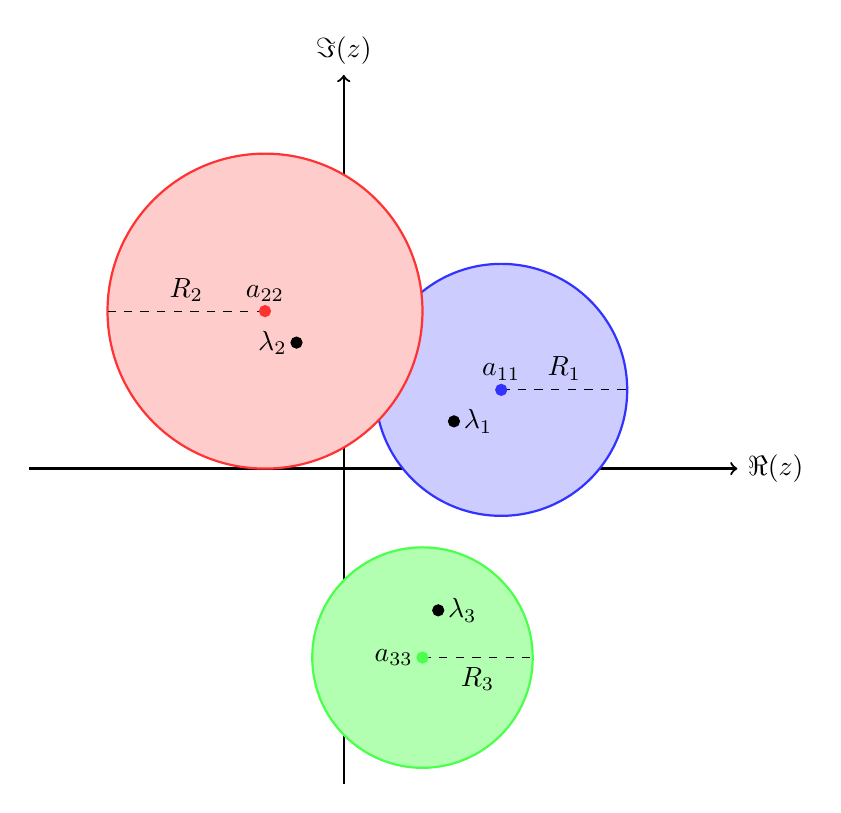
\begin{tikzpicture}[scale=2.0]
  % Axes
  \draw[->,thick] (-2,0) -- (2.5,0) node[right] {$\Re(z)$};
  \draw[->,thick] (0,-2) -- (0,2.5) node[above] {$\Im(z)$};

  % Define diagonal entries (centers of discs)
  \coordinate (a11) at (1,0.5);
  \coordinate (a22) at (-0.5,1);
  \coordinate (a33) at (0.5,-1.2);

  % Draw Gershgorin discs with different colors
  \filldraw[blue!20, draw=blue!80, thick] (a11) circle (0.8);
  \filldraw[red!20, draw=red!80, thick] (a22) circle (1);
  \filldraw[green!30, draw=green!70, thick] (a33) circle (0.7);

  % Draw radii with labels
  \draw[black, dashed] (a11) -- ++(0.8,0) node[black, midway, above] {$R_1$};
  \draw[black, dashed] (a22) -- ++(-1,0) node[black,midway, above] {$R_2$};
  \draw[black, dashed] (a33) -- ++(0.7,0) node[black,midway, below] {$R_3$};

  % Mark centers (diagonal entries)
  \filldraw[blue!80] (a11) circle (1pt) node[above,black] {$a_{11}$};
  \filldraw[red!80] (a22) circle (1pt) node[above,black] {$a_{22}$};
  \filldraw[green!70] (a33) circle (1pt) node[left, black] {$a_{33}$};

  % Mark some eigenvalues inside the region
  \filldraw[black] (0.7,0.3) circle (1pt) node[right] {$\lambda_1$};
  \filldraw[black] (-0.3,0.8) circle (1pt) node[left] {$\lambda_2$};
  \filldraw[black] (0.6,-0.9) circle (1pt) node[right] {$\lambda_3$};

\end{tikzpicture}
    \caption{Gershgorin discs $D_i$ in the complex plane. Each eigenvalue must lie within at least one disc. Isolated disc clusters contain a number of eigenvalues equal to the number of discs in the cluster.}
    \label{fig:gershgorin-discs}
\end{figure}

\paragraph{Irreducible matrices.}
A matrix $A$ is \emph{irreducible} if its directed graph is strongly connected, or equivalently, no permutation reduces $A$ to block upper-triangular form with a zero block below the diagonal. For irreducible matrices, if any eigenvalue lies on the boundary of one disc, it must lie on the boundary of \emph{all} discs—a strong global constraint.

\subsection{Diagonal Dominance and Nonsingularity}\label{subsec:diagonal-dominance}

A matrix $A$ is \emph{strictly diagonally dominant by rows} if
\[
    |a_{ii}| > R_i \qquad \text{for all } i=1,\dots,n.
\]
Geometrically, this means each Gershgorin disc $D_i$ excludes the origin.

\paragraph{Levy–Desplanques theorem.} If $A$ is strictly diagonally dominant, then $A$ is nonsingular.

\begin{proof}[Proof]
    Since $0\notin D_i$ for any $i$, Gershgorin's theorem implies $0\notin\sigma(A)$.
\end{proof}

\paragraph{Varga's criterion (irreducible case).} If $A$ is irreducible and weakly diagonally dominant ($|a_{ii}|\ge R_i$ for all $i$) with strict inequality for at least one row, then $A$ is nonsingular.

\begin{proof}[Proof sketch]
    If $0$ were an eigenvalue, irreducibility forces $0$ to lie on the boundary of all discs. But at least one disc strictly excludes the origin, a contradiction.
\end{proof}

\paragraph{Perturbation insight.} Consider the homotopy $A(t)=D+tH$. At $t=0$, eigenvalues coincide with diagonal entries; as $t\to 1$, they move continuously within shrinking discs. This perspective explains why diagonal dominance stabilizes spectra under perturbations and why iterative methods (which implicitly reduce off-diagonal coupling) drive eigenvalues toward diagonal entries.

\end{document}